
\section{Modelos de Regresion}

Finalmente, vemos los modelos propuestos. Primero sin la libertad mundial como independiente, y luego con está. Los resultados se muestran en la Tabla %\ref{regresiones} de la página \pageref{regresiones}.




% Table created by stargazer v.5.2.2 by Marek Hlavac, Harvard University. E-mail: hlavac at fas.harvard.edu
% Date and time: vie., jun. 29, 2018 - 9:13:58 p.m.
\begin{table}[!htbp] \centering 
  \caption{Modelo de regresi�n propuesto para los datos de departamentos de cabecera} 
  \label{stats} 
\begin{tabular}{@{\extracolsep{5pt}}lc} 
\\[-1.8ex]\hline 
\hline \\[-1.8ex] 
 & \multicolumn{1}{c}{\textit{Dependent variable:}} \\ 
\cline{2-2} 
\\[-1.8ex] & IDH \\ 
\hline \\[-1.8ex] 
 cabeLog & 0.013$^{***}$ \\ 
  & (0.004) \\ 
  & \\ 
 Constant & 0.634$^{***}$ \\ 
  & (0.055) \\ 
  & \\ 
\hline \\[-1.8ex] 
Observations & 32 \\ 
R$^{2}$ & 0.238 \\ 
Adjusted R$^{2}$ & 0.212 \\ 
Residual Std. Error & 0.037 (df = 30) \\ 
F Statistic & 9.347$^{***}$ (df = 1; 30) \\ 
\hline 
\hline \\[-1.8ex] 
\textit{Note:}  & \multicolumn{1}{r}{$^{*}$p$<$0.1; $^{**}$p$<$0.05; $^{***}$p$<$0.01} \\ 
\end{tabular} 
\end{table} 
% Table created by stargazer v.5.2.2 by Marek Hlavac, Harvard University. E-mail: hlavac at fas.harvard.edu
% Date and time: vie., jun. 29, 2018 - 9:13:58 p.m.
\begin{table}[!htbp] \centering 
  \caption{Modelo de regresi�n propuesto para los datos de todos los departamentos} 
  \label{stats} 
\begin{tabular}{@{\extracolsep{5pt}}lc} 
\\[-1.8ex]\hline 
\hline \\[-1.8ex] 
 & \multicolumn{1}{c}{\textit{Dependent variable:}} \\ 
\cline{2-2} 
\\[-1.8ex] & IDH \\ 
\hline \\[-1.8ex] 
 cabeLog & 0.031$^{***}$ \\ 
  & (0.007) \\ 
  & \\ 
 restoLog & $-$0.030$^{***}$ \\ 
  & (0.010) \\ 
  & \\ 
 Constant & 0.766$^{***}$ \\ 
  & (0.065) \\ 
  & \\ 
\hline \\[-1.8ex] 
Observations & 32 \\ 
R$^{2}$ & 0.425 \\ 
Adjusted R$^{2}$ & 0.385 \\ 
Residual Std. Error & 0.033 (df = 29) \\ 
F Statistic & 10.706$^{***}$ (df = 2; 29) \\ 
\hline 
\hline \\[-1.8ex] 
\textit{Note:}  & \multicolumn{1}{r}{$^{*}$p$<$0.1; $^{**}$p$<$0.05; $^{***}$p$<$0.01} \\ 
\end{tabular} 
\end{table} 


Como se vio en la Tabla %\ref{regresiones}, cuando está presente el \emph{indice de libertad mundial}, el \emph{�?ndice de libertad de prensa} pierde significancia.
\begin{Schunk}
\begin{Soutput}
OGR data source with driver: ESRI Shapefile 
Source: "D:\Documentos\Repositorios\ProyectoFinal\COL_maps\COL_adm1.shp", layer: "COL_adm1"
with 32 features
It has 9 fields
Integer64 fields read as strings:  ID_0 ID_1 
\end{Soutput}
\begin{Soutput}
[1] 1 3 2
\end{Soutput}
\begin{Soutput}
  Group.1       IDH  cabeLog restoLog
1       1 0.7607000 11.24731 11.25763
2       2 0.8175455 13.42100 12.10201
3       3 0.8235455 14.27185 13.42408
\end{Soutput}
\end{Schunk}
\begin{figure}
\centering
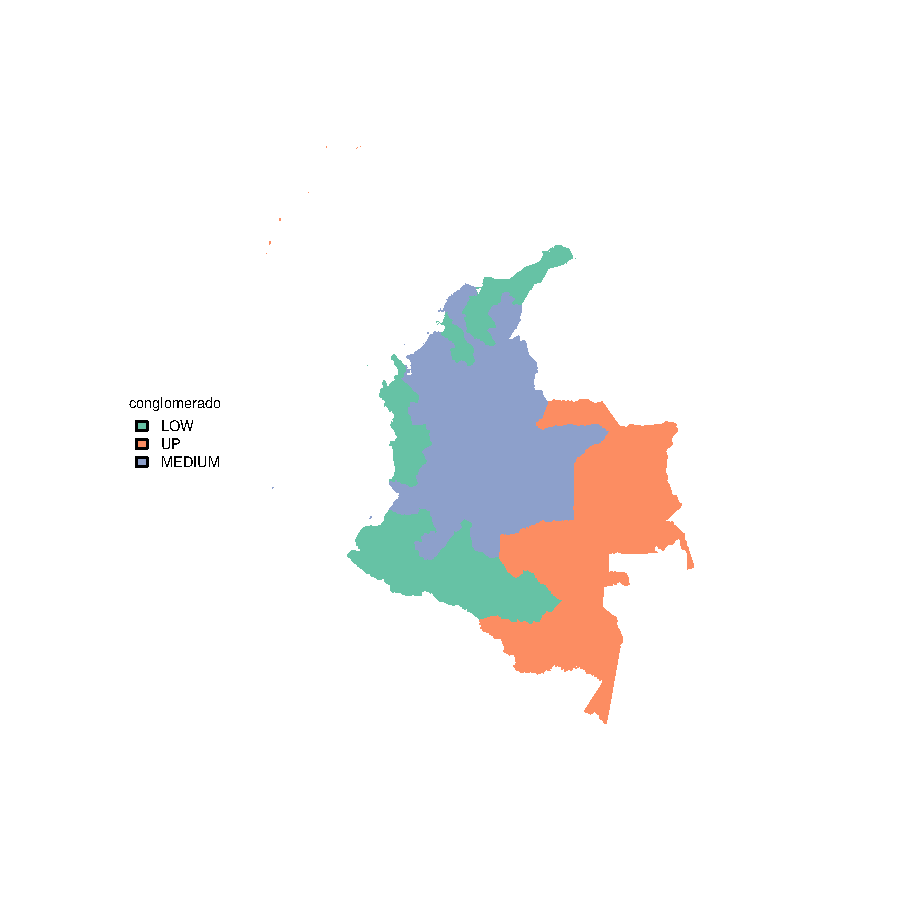
\includegraphics{Modelos_regresion-plotMap1}
\caption{Histograma del IDH en Colombia para los 32 departamentos}
\label{mapa}
\end{figure}
\endinput
